\section{Введение}
\begin{frame}{Введение}
    \begin{itemize}
        \item Конструктивизм --- авангардистское направление в искусстве, зародившиеся в 1920 --- 1930 годах в СССР.
              \pause
        \item Конструктивизм оказал значительное влияние на архитектуру, в том числе и на современную
              \begin{figure}
                  \centering
                  \begin{subfigure}[b]{0.45\textwidth}
                      \centering
                      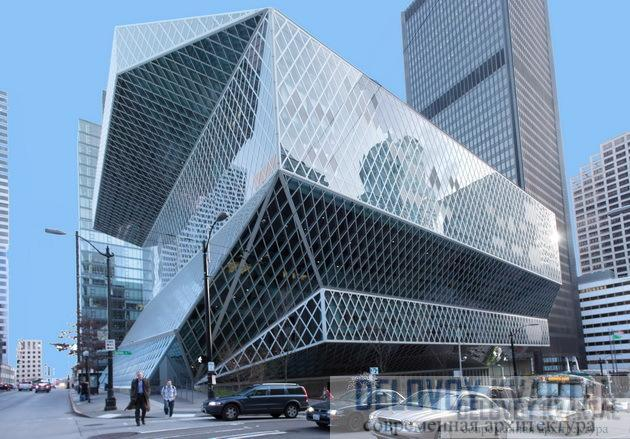
\includegraphics[height=3cm]{images/seattle.jpg}
                      \caption*{Центральная библиотека Сиэтла \\ Сиэтл, штат Вашингтон, США}
                  \end{subfigure}
                  \hfill
                  \begin{subfigure}[b]{0.45\textwidth}
                      \centering
                      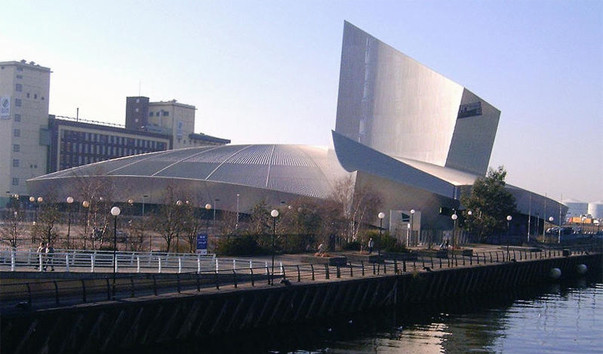
\includegraphics[height=3cm]{images/iwms.jpg}
                      \caption*{Имперский военный музей Севера \\ Манчестер, Великобритания}
                  \end{subfigure}
              \end{figure}
              \pause
        \item  А также на книжную графику, дизайн костюмов,
        \texttt{и даже на дизайн шрифтов}
    \end{itemize}

\end{frame}